% !TEX root = ../presentation.tex
% !BIB program = biber
% !TEX program = xelatex

\section[A Brief Overview of Unsupervised Speech Representation Learning]{a brief overview of unsupervised speech representation learning}


\begin{frame}
    \frametitle{Overview: Representation Learning for Speech}

    \begin{columns}

        \begin{column}{0.4\textwidth}
            \begin{itemize}
                \item Reviews two learning paradigms:
                \begin{itemize}
                    \item Self-supervised learning (SSL)
                    \item Probabilistic latent variable models (LVMs)
                \end{itemize}
                \item Recent developments have been driven by \highlight{self-supervised learning}.
                \item A model-by-model overview for selected self-supervised models.
            \end{itemize}
        \end{column}

        \begin{column}{0.6\textwidth}
            \begin{tikzpicture}
                \only<1->{
                    \node[anchor=south west,inner sep=0] (A) at (0,0) {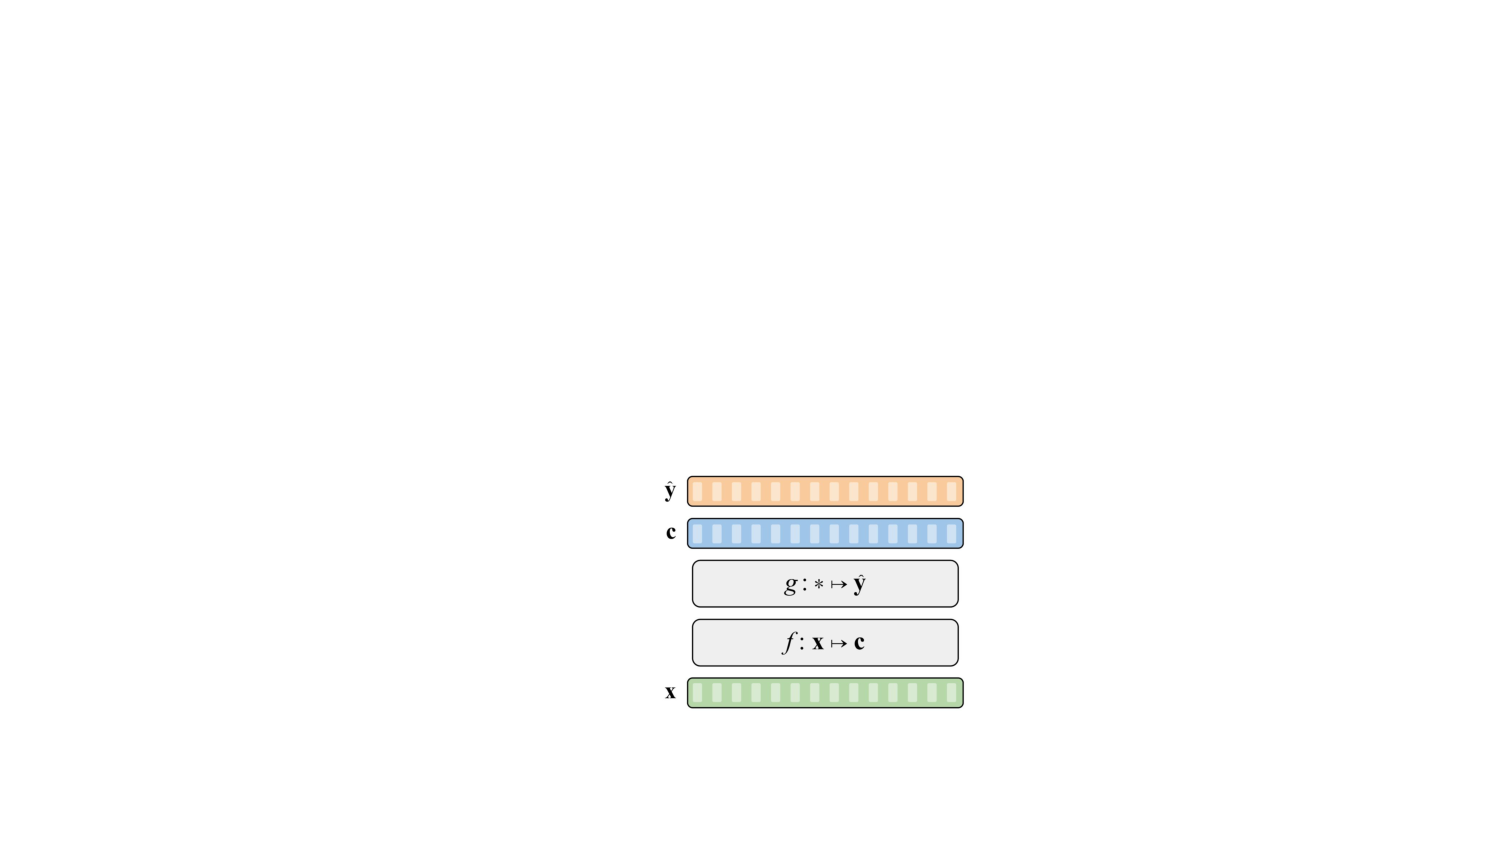
\includegraphics[height=0.4\textheight]{figures/brief-paradigms-ssl.pdf}};
                    \node[anchor=south west,inner sep=0] (B) at (4.2,0) {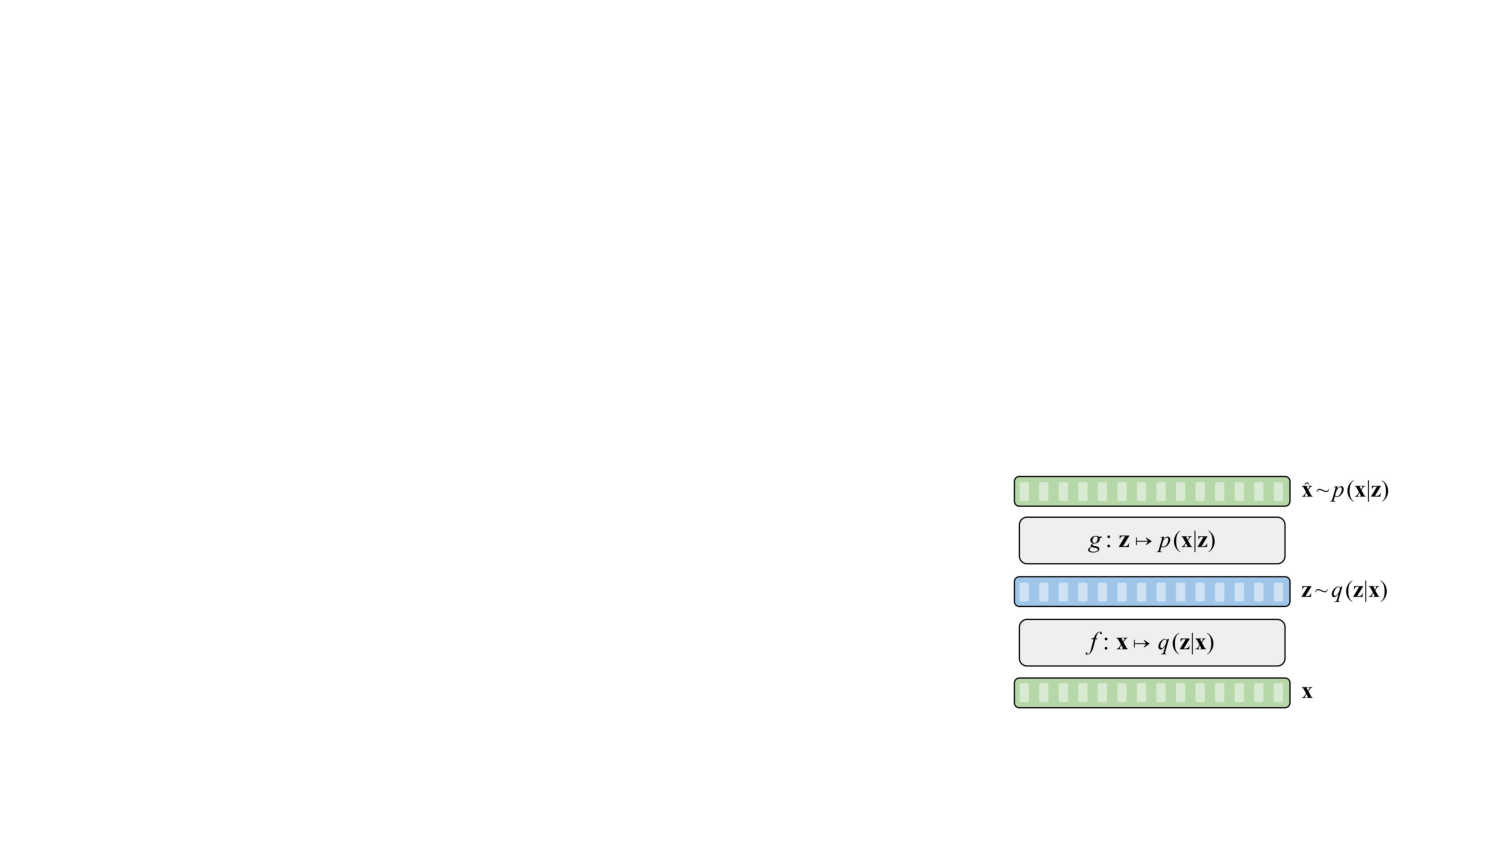
\includegraphics[height=0.4\textheight]{figures/brief-paradigms-lvm-2.pdf}};
                }
            
                \only<2->{
                    \node[anchor=south west,inner sep=0] (A) at (0,0) {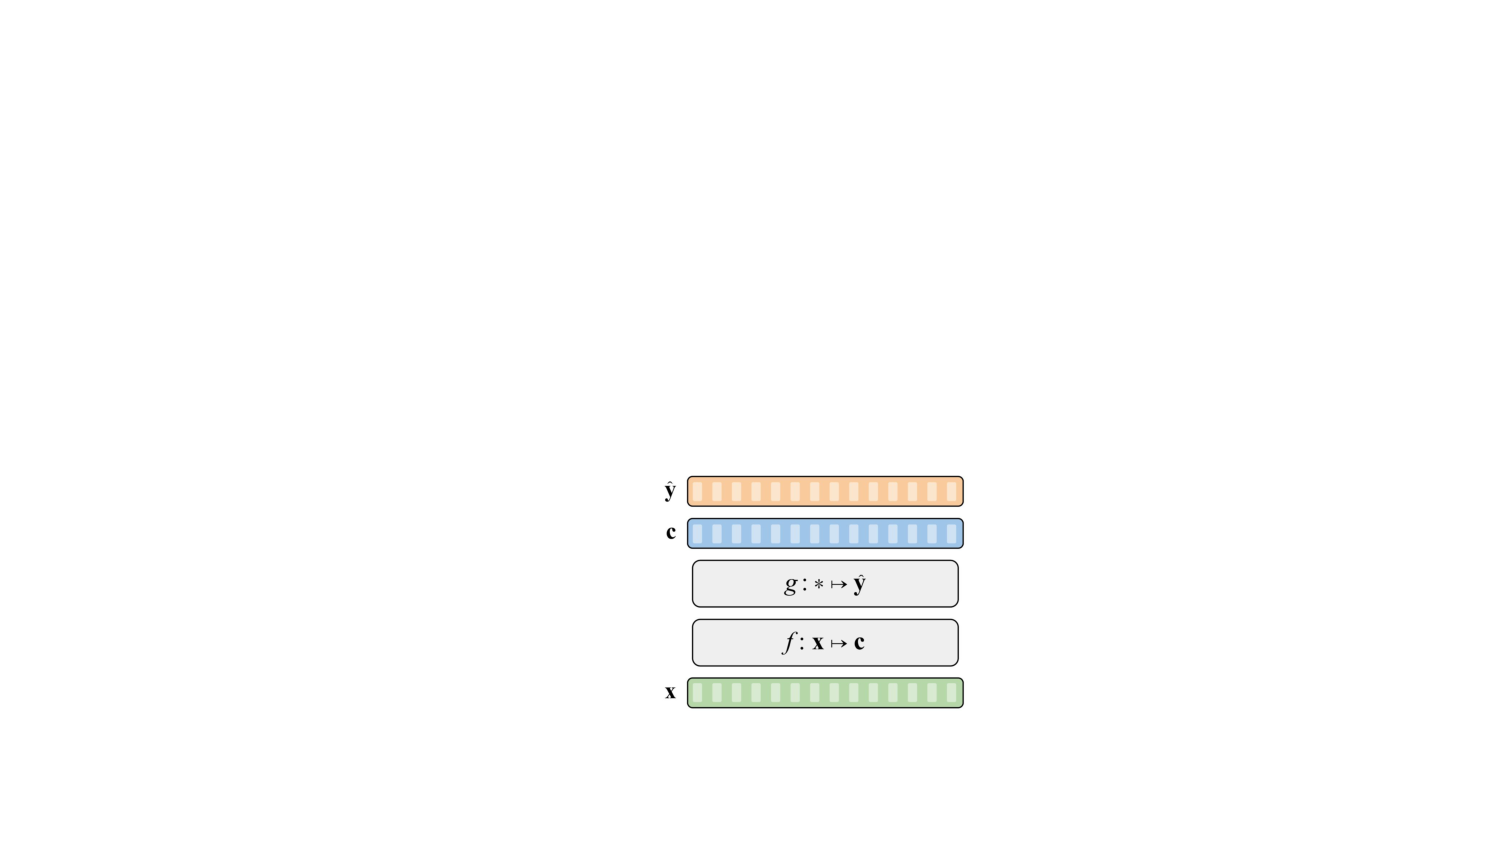
\includegraphics[height=0.4\textheight]{figures/brief-paradigms-ssl.pdf}};
                    \node[anchor=south west,inner sep=0] (B) at (4.2,0) {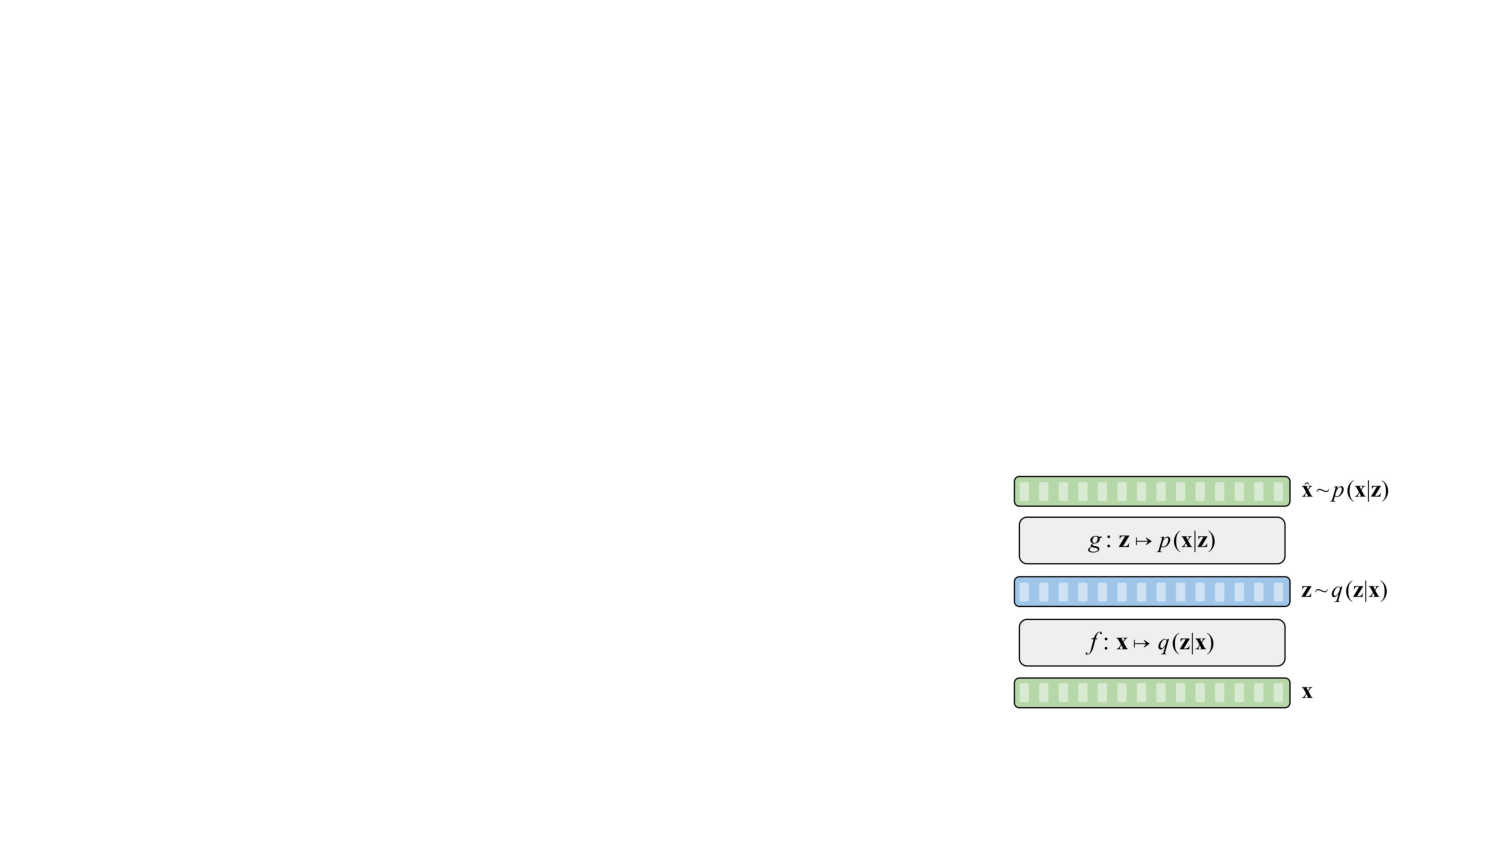
\includegraphics[height=0.4\textheight]{figures/brief-paradigms-lvm-2.pdf}};
                    \fill [draw=none, fill=white, fill opacity=0.7] (B.north west) -- (B.north east) -- (B.south east) -- (B.south west) -- (B.north west) -- cycle;
                }
            \end{tikzpicture}
        \end{column}
    \end{columns}

    \note[item]{Focus on the self-supervised learning models.}
\end{frame}


\begin{frame}
    \frametitle{\vphantom{ABCDEFGHJIJKLMNOPQRSTVWXYZ}{Development of SSL for speech}}
    \begin{columns}[t]
        \hspace{0.025\textwidth}
        \begin{column}{0.20\textwidth}
            \begin{figure}[\textwidth]
                \centering
                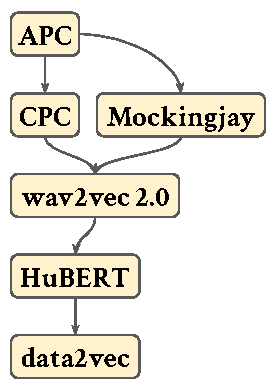
\includegraphics[width=\textwidth]{figures/brief-flow-0.pdf}
            \end{figure}
        \end{column}
        {\textcolor{black!40}{\vrule{}}}
        \begin{column}{0.40\textwidth}
            {\vspace{0.10\textheight}\footnotesize
            \begin{itemize}
                \item \highlight{Common setup}: Learn representations from raw audio without supervision.
                \item \highlight{Main evaluation}: Speech recognition performance.
            \end{itemize}
            }
        \end{column}
        \begin{column}{0.30\textwidth}
            \begin{figure}[2.333\textwidth]
                % \centering
                % 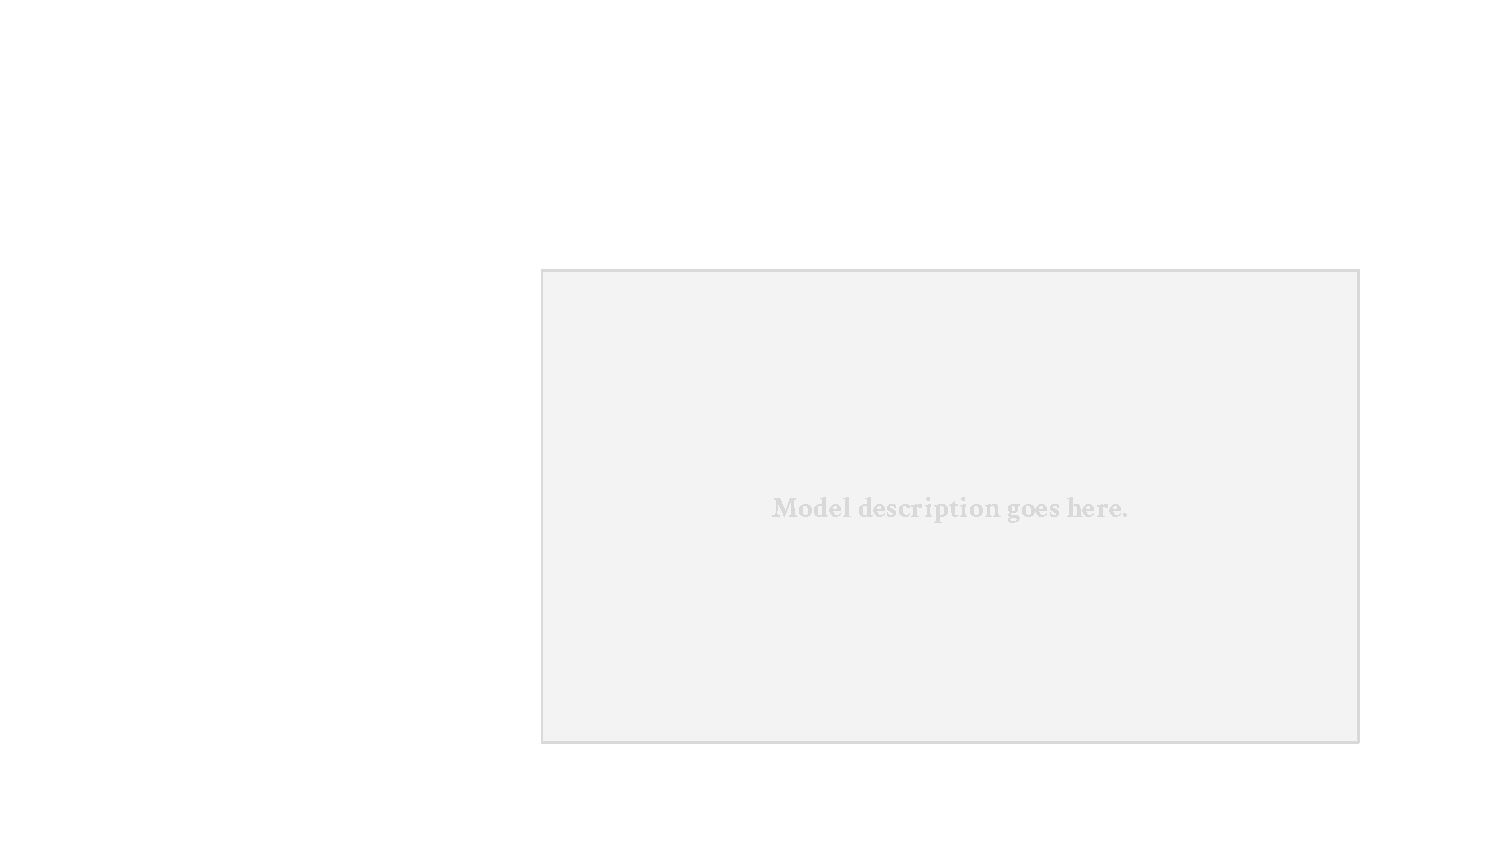
\includegraphics[width=2.333\textwidth]{figures/brief-model-0.pdf}
            \end{figure}
        \end{column}
        % \hspace{0.020\textwidth}
        % \begin{column}{0.70\textwidth}
        %     \centering
        %     \begin{figure}[\textwidth]
        %         \centering
        %         {\vspace{0.2\textheight}\color{black!40}\scshape model description goes here}
        %     \end{figure}
        % \end{column}
        \hspace{0.020\textwidth}
    \end{columns}
\end{frame}


{ % start font size change group

\setbeamerfont*{itemize/enumerate body}{size=\fontsize{8}{10}}
\setbeamerfont*{itemize/enumerate subbody}{parent=itemize/enumerate body}
\setbeamerfont*{itemize/enumerate subsubbody}{parent=itemize/enumerate body}

\newcommand{\presentationbriefslide}[3]{%
    \begin{frame}
        \frametitle{\vphantom{ABCDEFGHJIJKLMNOPQRSTVWXYZ}{#2}}
        \begin{columns}[t]
            \hspace{0.025\textwidth}
            \begin{column}{0.20\textwidth}
                \begin{figure}[\textwidth]
                    \centering
                    \includegraphics[width=\textwidth]{figures/brief-flow-#1.pdf}
                \end{figure}
            \end{column}
            {\textcolor{black!40}{\vrule{}}}
            \begin{column}{0.40\textwidth}
                {\vspace{0.10\textheight}\footnotesize#3}
            \end{column}
            \begin{column}{0.30\textwidth}
                \begin{figure}[\textwidth]
                    \centering
                    \includegraphics[width=\textwidth]{figures/brief-model-#1.pdf}
                \end{figure}
            \end{column}
            \hspace{0.020\textwidth}
        \end{columns}
    \end{frame}
}

% \presentationbriefslide{0}{Development of SSL for speech}{}%

\presentationbriefslide{1}{Autoregressive Predictive Coding (APC)}{%
    \begin{itemize}
        \item {\bfseries \color{black} Task}: Predict future inputs.
        \item {\bfseries \color{black} Input/target}: Log-mel spectrogram.
        \item {\bfseries \color{black} Architecture}: RNN/Transformer decoder.
        \item {\bfseries \color{black} Slow features}: Predict $k$ steps ahead.
    \end{itemize}
}

\presentationbriefslide{2}{Autoregressive Predictive Coding (APC)}{%
    \begin{itemize}
        \item {\bfseries \color{black} Challenges}:
        \begin{itemize}
            \item Encodes only past inputs \xmark
            \item Uses the input as target \xmark
        \end{itemize}
    \end{itemize}

    \note[item]{Encoding only past inputs limits the model's ability to learn from future context.}
    \note[item]{Input as target limits the model's ability to learn abstract representations.}
}

\presentationbriefslide{3}{Mockingjay}{%
    \begin{itemize}
        \item {\bfseries \color{black} Task}: Reconstruct masked inputs.
        \item {\bfseries \color{black} Architecture}: Transformer encoder.
        \item {\bfseries \color{black} Masking}: 
        \begin{itemize}
            \item $X$\% at random. (Mockingjay)
            \item $X$\% + $N$ consecutive (wav2vec 2.0)
            % \item SpecAugment (Masked RNN)
        \end{itemize}
    \end{itemize}

    \note[item]{Replaces autoregressiveness with a masked reconstruction task.}
    \note[item]{Masking strategy to force learning long-term context.}
}

\presentationbriefslide{4}{Mockingjay}{%
    \begin{itemize}
        \item {\bfseries \color{black} Challenges}:
        \begin{itemize}
            \item Encodes the entire input \cmark
            \item Uses the input as target \xmark
        \end{itemize}
    \end{itemize}
}

\presentationbriefslide{5}{Contrastive Predictive Coding (CPC)}{%
    \begin{itemize}
        \item {\bfseries \color{black} Contrastive learning}: Distinguish target samples from negative samples.
        \item {\bfseries \color{black} Learned target}: Discard details.
        \item {\bfseries \color{black} Sampling negatives}:
        \begin{itemize}
            \item Same sequence?
            \item Same speaker?
        \end{itemize}
    \end{itemize}

    \note[item]{Contrastive models allow using a learned target. Discard unimportant details of input.}
    \note[item]{Negative sampling is a challenge and requires careful design.}
    \note[item]{Sampling different speakers as negatives learns strong speaker-identities.}
}

\presentationbriefslide{6}{Contrastive Predictive Coding (CPC)}{%
    \begin{itemize}
        \item {\bfseries \color{black} Challenges}:
        \begin{itemize}
            \item <1-> Only encodes past inputs \xmark
            \item <1-> Uses a learned target \cmark
            \item <2-> Sampling negatives \xmark
        \end{itemize}
    \end{itemize}
}

\presentationbriefslide{8}{wav2vec 2.0} WER.
            \item 10 minutes: \textbf{4.8\%} WER.
        \end{itemize}
    \end{itemize}

    \note[item]{Training objective requires identifying the correct quantized latent audio representation in a set of distractors for each masked time step.}
    \note[item]{Quantisation improves negative sampling (requires approximation via Gumbel softmax).}
}

\presentationbriefslide{9}{wav2vec 2.0}{%
    \begin{itemize}
        \item {\bfseries \color{black} Challenges}:
        \begin{itemize}
            \item Encodes the entire input \cmark
            \item Uses a learned target \cmark
            \item Sampling negatives \xmarkshaded
        \end{itemize}
    \end{itemize}
}

\presentationbriefslide{10}{Hidden-unit BERT (HuBERT)}{%
    \begin{itemize}
        \item {\bfseries \color{black} Target}: $K$-means teacher (MFCC frames).
        \item {\bfseries \color{black} Training}: Cross-entropy loss.
        \item {\bfseries \color{black} 1st iteration}: $K$-means on inputs.
    \end{itemize}

    \note[item]{HuBERT approach predicts hidden cluster assignments of masked frames}
}


\presentationbriefslide{11}{Hidden-unit BERT (HuBERT)}{%
    \begin{itemize}
        \item {\bfseries \color{black} Target}: $K$-means teacher (MFCC frames).
        \item {\bfseries \color{black} Training}: Cross-entropy loss.
        \item {\bfseries \color{black} 1st iteration}: $K$-means on inputs.
        \item {\bfseries \color{black} 2nd iteration}: $K$-means on hidden layers.
    \end{itemize}

    \note[item]{HuBERT approach predicts hidden cluster assignments of masked frames}
}


\presentationbriefslide{12}{Hidden-unit BERT (HuBERT)}{%
    \begin{itemize}
        \item {\bfseries \color{black} Challenges}:
        \begin{itemize}
            \item <1-> Encodes the entire input \cmark
            \item <1-> Uses a learned target \cmark
            \item <1-> No need for negative samples \cmark
            \item <2-> Targets updated infrequently \xmark
            \item <2-> Quantized targets \xmark
        \end{itemize}
    \end{itemize}

    \note[item]{HuBERT approach predicts hidden cluster assignments of masked frames}
    \note[item]{Targets are still quantised although we no longer solve a contrastive sampling problem. Might reduce quality.}
}

\presentationbriefslide{14}{data2vec}{%
    \begin{itemize}
        \item Uses a teacher-student framework.
        \item {\bfseries \color{black} Teacher}:
        \begin{itemize}
            \item EMA of student (online) \cmark
            \item Target is average of top $K$ layers \cmark
        \end{itemize}
    \end{itemize}
}

\presentationbriefslide{15}{data2vec}{%
    \begin{itemize}
        \item Uses a teacher-student framework.
        \item {\bfseries \color{black} Teacher}:
        \begin{itemize}
            \item EMA of student (online) \cmark
            \item Target is average of top $K$ layers \cmark
        \end{itemize}
        \item {\bfseries \color{black} Student training}: Smooth $\ell_1$ loss.
    \end{itemize}
}

\presentationbriefslide{16}{data2vec}{%
    \begin{itemize}
        \item {\bfseries \color{black} Challenges}:
        \begin{itemize}
            \item Encodes the entire input \cmark
            \item Uses a learned target \cmark
            \item No need for negative samples \cmark
            \item Targets updated continuously \cmark
            \item Continuous-valued targets \cmark
        \end{itemize}
    \end{itemize}
}


} % end font size change group

\begin{frame}
    \frametitle{Conclusions}
    \begin{itemize}
        \item {\bfseries Main conclusions}:
        \begin{itemize}
            \item The most popular self-supervised speech models can be compactly described by a few core design choices.
            \item Many of these design choices are mirrored in earlier work on speech embedding models.
        \end{itemize}
        \item {\bfseries Open questions and limitations}:
        \begin{itemize}
            \item Which design choices benefit which downstream tasks?
            \item It is difficult to compare methods as model size and evaluation procedures differ widely between papers.
        \end{itemize}
    \end{itemize}

    \note[item]{Predictive, Contrastive, Masking, Learned targets, Quantization, Teacher-student}
    \note[item]{Audio Word2vec, Speech2Vec, Unspeech which also used masking, and predictive and contrastive setups.}
\end{frame}
